\chapter{Partitioning}

\textbf{Partitioning} becomes necessary when dealing with \textbf{large data sets} and high \textbf{query throughput}. It is a technique that divides a large data set into smaller, more manageable parts. This is done to improve the performance of the system. Partitioning can be done in various ways, such as horizontal partitioning, vertical partitioning, and functional partitioning. In this chapter, we will discuss the different types of partitioning and their benefits.

``Partition'' is the most common term, but it may vary depending on the technology:
\begin{itemize}
   \item \textbf{Shard} in MongoDB, Elasticsearch, and Cassandra.
   \item \textbf{Region} in HBase.
   \item \textbf{VBucket} in Couchbase.
   \item \textbf{Tablet} in Bigtable.
   \item \textbf{VNode} in Riak and Cassandra.	
\end{itemize} 

\section{Partitioning concepts}
First, partitions must be \textbf{defined}, in the sense that each piece of data must be assigned to a partition. This can be done in various ways, such as hashing, range partitioning, or list partitioning.

Then, each partition should have its own \textbf{characteristics}, i.e. should support a known set of operations, since it acts as a small per se database.

Clearly, different partitions may reside on different nodes, enabling scalability.


\subsection{Combining partitioning with replication}

\begin{paracol}{2}
   \colfill
   Partitioning can be combined with replication to improve the performance and reliability of the system. Replication is the process of creating multiple copies of the data and storing them on different nodes. This ensures that the data is available even if one of the nodes fails. \ul{By combining partitioning with replication, you can achieve high availability and fault tolerance.}
   \colfill
   
   \switchcolumn

   \begin{figure}[htbp]
      \centering
      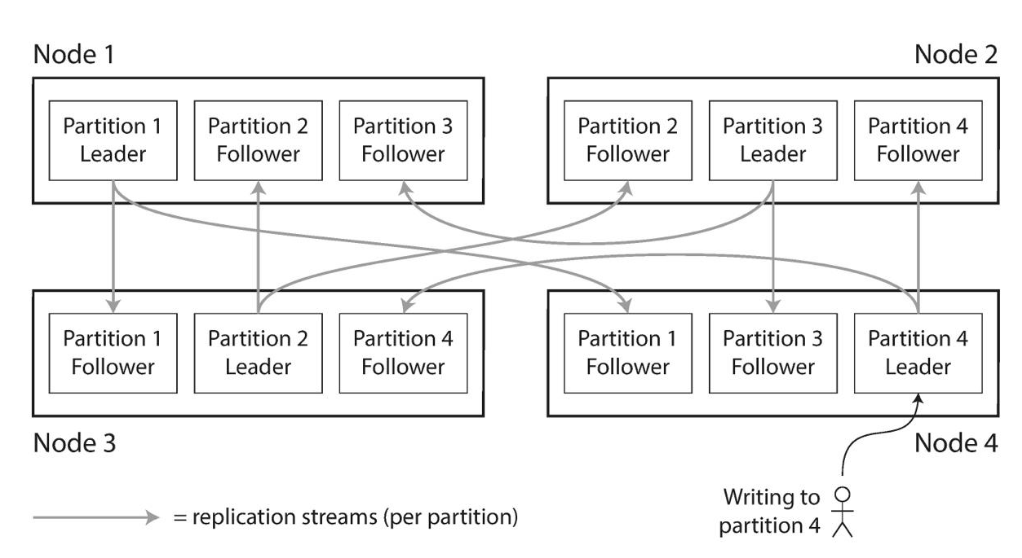
\includegraphics[width=0.95\columnwidth]{images/11/leader_follower.png}
      \caption{Leader-follower model}
      \label{fig:11/leader_follower}
   \end{figure}
\end{paracol}

This can be achieved in various ways:
\begin{enumerate}
   \item Node Storage of Multiple Partitions
   \begin{itemize}
      \item Nodes can store more than one partition, and \ul{each partition can be stored on multiple nodes}.
   \end{itemize}
   \item \textbf{Leader} and \textbf{Follower} assignment
   \begin{itemize}
      \item Each node stores a partition, and one of the nodes is designated as the leader. The leader is responsible for handling all write operations, while the followers replicate the data from the leader.
   \end{itemize}
   \item Replication and Partitioning
   \begin{itemize}
      \item The two techniques are enforced independently.
   \end{itemize}
\end{enumerate}

The Goal of partitioning is to spread data and query load \textbf{evenly} among the nodes.
Unfair partitioning can lead to \textbf{hot spots}, where some nodes are overloaded while others are underutilized.\\
Randomizing the partitioning function can help to avoid hot spots, but it can also make it difficult to locate data, requiring to query all nodes to get a value.

\subsection{Key-Range Partitioning}
A first improvement might be to provide a range-key assignment allowing to locate data, as it happens in libraries, where books are ordered by author or title.\\
In this way you know the boundaries of where to search. This is very easy to implement and to understand,
however, it is \textit{not} optimal:
\ul{data may \textbf{not} be evenly distributed among the possible keys}.

\section{Avoiding Hot spots}
So with key-range partitioning, the problem is that some keys may be more popular than others due to access patterns, leading to hot spots.\\
In, for instance, a sensor database, all today's writes would end up in the same ``today's partition'', while the rest of the partitions would be idle.
\nl

A solution might be to change-key structure, for instance by adding a prefix to the key, such as the sensor ID, to distribute the data more evenly.

\subsection{Hash partitioning}
A better solution is to use \textbf{hash partitioning}, where a hash function is used to map keys to partitions.\\
However we must be careful because \textbf{inconsistent} hashing can lead to hot spots, as the hash function may not distribute keys evenly.

Note also that hash partitioning is very bad for range queries, as even similar data is spread randomly across the partitions.

\subsubsection{Secondary Indexes}
% Copilot generated
Secondary indexes are a way to avoid hot spots in hash partitioning.\\
The idea is to create a separate index that maps the secondary key to the primary key, and then use the primary key to locate the data.\\
This way, the secondary key is hashed and distributed evenly across the partitions, while the primary key is used to locate the data.


\begin{itemize}
   \item \textbf{Document}-based partitioning (local indexes)
   \begin{itemize}
      \item Each listing has a unique document ID
      \item Database is partitioned based on the document ID
      \item Secondary indexes are on fields like color and make
      \item \ul{\textit{Reading} requires querying all partitions}
   \end{itemize}
   \item \textbf{Term}-based partitioning (global indexes)
   \begin{itemize}
      \item A Global index covers data in all partitions.
      \item Partitioning is based on the term ID, which is not the primary key index.
      \item 
   \end{itemize}
\end{itemize}

\section{Rebalancing}
Rebalancing is the process of moving data between partitions to ensure that the data is evenly distributed among the nodes. This is necessary when the data distribution changes, for example, when new nodes are added to the system or when the data distribution becomes uneven due to hot spots. Rebalancing can be done in various ways, such as automatic rebalancing, manual rebalancing, and dynamic rebalancing.

\framedt{Challenges in rebalancing}{
   \begin{itemize}
      \item Fair load distribution
      \item Continuous operation during rebalancing
      \item Minimizing data movement
   \end{itemize}
}

\subsection{Optimizing rebalancing - Kademlia and P2P recalls}

Assigning keys to nodes computing $h(key) mod \#{nodes} \rightarrow node$ is intuitive but leads to a tremendous amount of data movement when nodes are added or removed, since all modulo values must be recomputed.\\
A better solution is to use a \textbf{distributed hash table} (DHT) such as \textbf{Kademlia} or \textbf{Chord}, which allows to find the node responsible for a key in $O(\log n)$ steps.

A simple intuition exploited by both Kademlia and Chord is to fix the granularity of the keyspace prior to partitioning.

In other words, having a fixed number of partitions may help to avoid data movement when nodes are added or removed.


\subsection{Dynamic partitioning}
Dynamic partitioning is a technique that allows the system to adapt to changes in the data distribution. This is done by monitoring the data distribution and rebalancing the data when necessary. Dynamic partitioning can be done in various ways, such as automatic rebalancing, manual rebalancing, and dynamic rebalancing.

\begin{itemize}
   \item \textbf{Automatic} rebalancing - System automatically rebalances the data when necessary without any human intervention.
   May be unpredictable and expensive, but requires less maintanance.
   \item \textbf{Manual} rebalancing - Administrator manually rebalances the data when necessary. May be better since and admin may have a more \textit{comprehensive} view of the distributed system, while a machine may be limited by network partitioning, discovery, etc.
   \item \textbf{Hybrid} approach - Combines automatic and manual rebalancing. The system automatically rebalances the data when necessary, but the administrator can override the system's decisions. 
\end{itemize}

\subsection{Routing}
Routing is the process of determining which partition to send a query to. This is done by either forwarding requests to a routing tier, or by having partition-aware clients which know how the data is distributed. Routing can be done in various ways, such as static routing, dynamic routing, and consistent hashing.



The opposite approach is to query all partitions, which is very expensive, but may be necessary in some cases.


\section{Takeaways}
Data partitioning enhances scalability by distributing data across multiple nodes, and when combined with replication, it can improve the performance and reliability of the system. However, partitioning can introduce challenges such as hot spots and rebalancing. To address these challenges, you can use techniques such as hash partitioning, secondary indexes, and dynamic partitioning. By carefully designing the partitioning strategy, you can achieve high availability, fault tolerance, and scalability in your system.